
\begin{figure}[t]
  \centering
  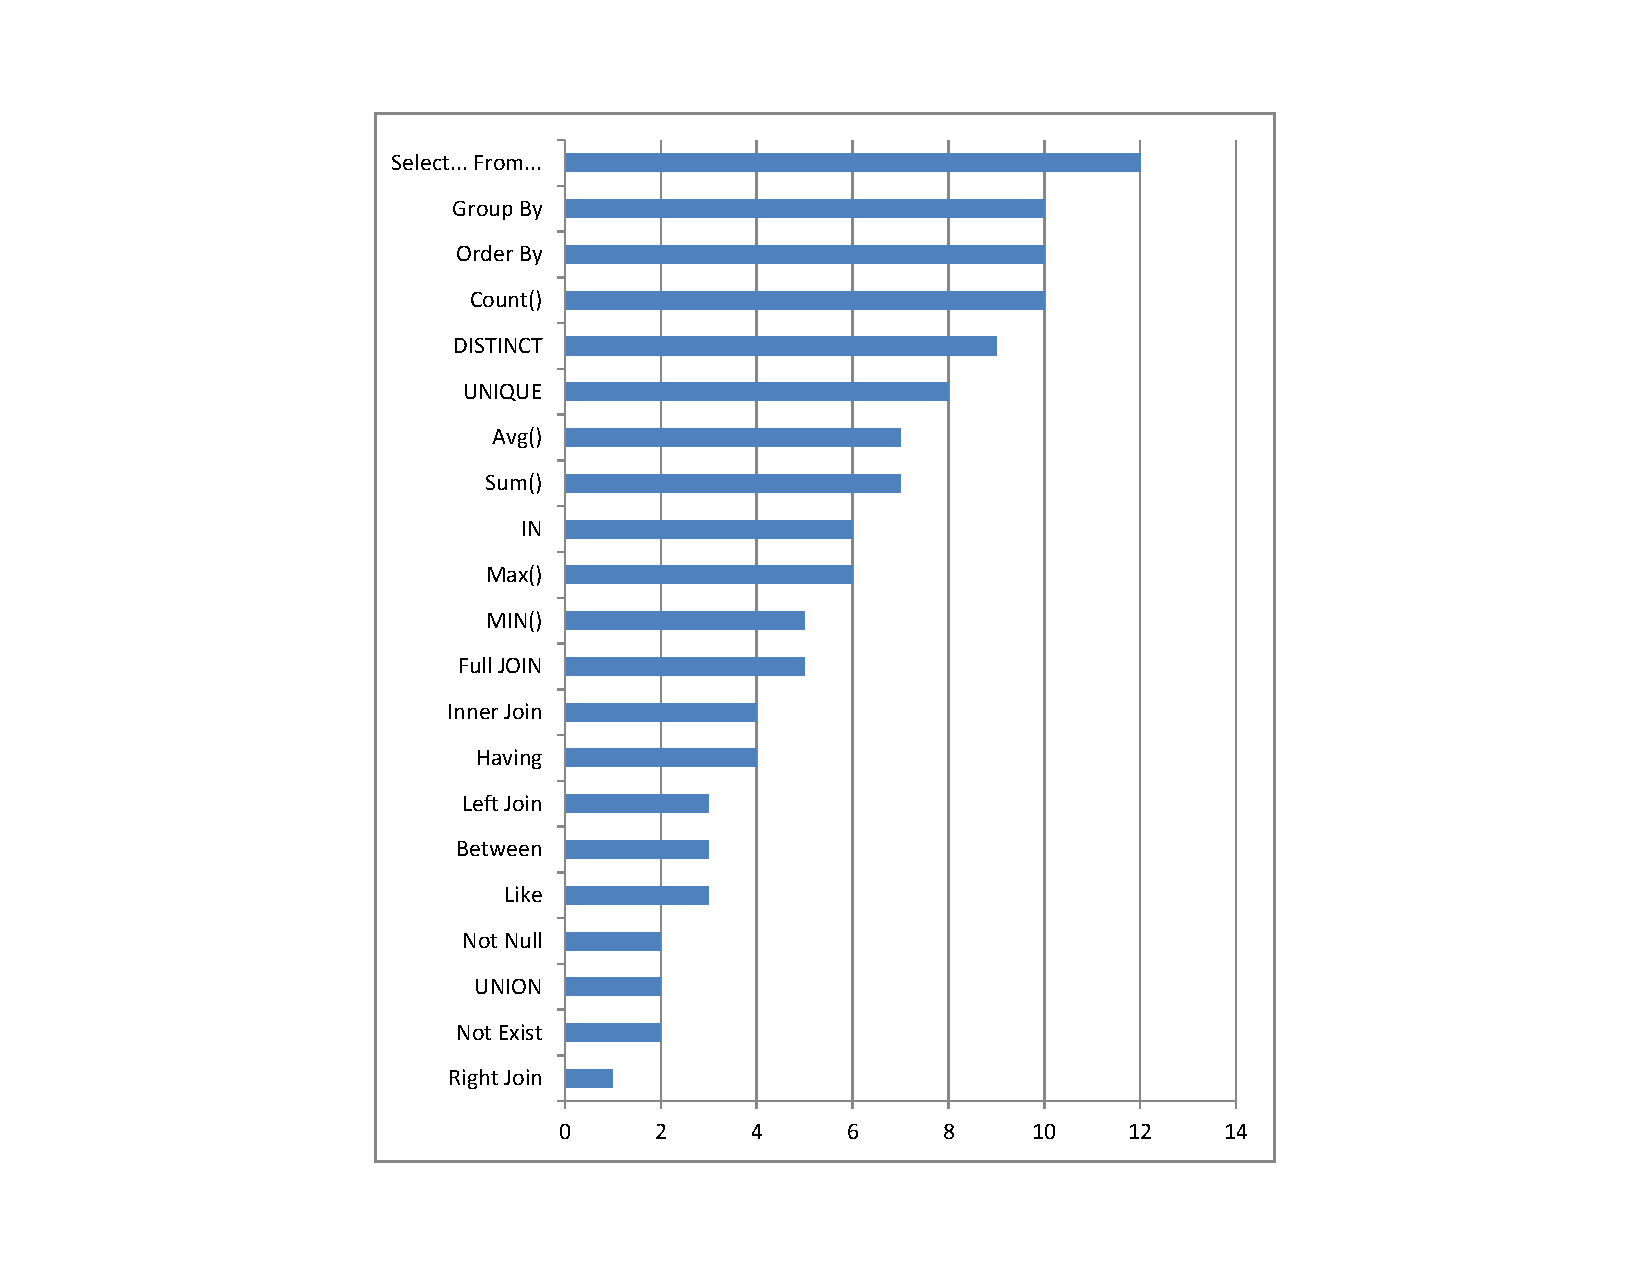
\includegraphics[scale=0.50]{survey}
  \vspace*{-1.0ex}\caption {{\label{fig:survey}
  Survey results of the most important SQL features
  in writing a database query. There were 12 participants
  in the survey, and each participant was asked to
  select the top 10 most important SQL features.
  SQL features with no selection \todo{x} are omitted for brevity.
}}

\end{figure}

\newcommand{\q}{\langle query\rangle}
\newcommand{\db}{\langle db\rangle}
\newcommand{\pat}{\langle pat\rangle}
\newcommand{\bug}{\langle bug\rangle}
\newcommand{\dist}{\langle distance\rangle}
\newcommand{\sem}[1]{\llbracket #1\rrbracket}
\newcommand{\lit}[1]{\texttt{#1}}

\newcommand{\column}{\langle column\rangle}
\newcommand{\dbtable}{\langle table\rangle}
\newcommand{\cond}{\langle cond\rangle}
\newcommand{\op}{\langle op\rangle}
\newcommand{\e}{\langle expr\rangle}
\newcommand{\ce}{\langle cexpr\rangle}

\begin{figure}[t]
%\scriptsize{%
\footnotesize%
\begin{align*}
\q ::= {} 
	& \texttt{ SELECT } \e^+ \texttt{ FROM } \dbtable^+ \\
        & \texttt{ WHERE } \cond^+ \\ 
	&  \texttt{ GROUP BY } \column^+ \texttt{ HAVING } \cond^+\\
	&  \texttt{ ORDER BY } \column^+ \\
\dbtable::= {} &\ atom \\
\column ::= {} &\ \dbtable.atom\\
\cond ::= {} &\ \ \cond \;\texttt{\&\&}\; \cond \\ 
    & |\ \cond \;\texttt{||}\; \cond \\
    & |\ \texttt{(}\;\cond\;\texttt{)} \\
    & |\ \ce \;\op\; \ce \\
    & |\ \texttt{NOT EXIST} \;(\q) \\
\op ::= {} &\ \ \texttt{=} \;\;|\;\; \texttt{>}  \;\;|\;\; \texttt{<}\\
\ce ::= {} &\ \ const \;\;|\;\; \column  \;\; \\
\e ::= {} & \ce \;\;|\ count(\column) \\
    & |\ sum(\column) \;\;|\ max(\column) \;\;|\ min(\column) 
\end{align*}
\normalsize%
\caption{Syntax of the supported SQL subset in \ourtool.
This subset covers the top XXX \todo{refer to figure 2}
in Figure~\ref{fig:survey}}
\label{fig:syntax}
\end{figure}


\section{Supported SQL Subset}
\label{sec:langsubset}


The full SQL language\footnote{Here, we refer to
the latest SQL 93 standard~\cite{}.} contains
\todo{.intractable.} keywords. It is infeasible to infer
the whole language\todo{revise}. Thus, the
first step is to identify a widely-used SQL
subset using which a large class of query tasks
can be performed. Unfortunately, no systematic
study has ever been conducted to this end,
and little empirical evidence has ever been provided
on which SQL features are important in practice.
Without such empirical knowledge, deciding which
SQL subset to support in \ourtool remains difficult.

\todo{Unlike some existing work, that the author decided
the language subset}

To address this issue, we first conducted an online survey
to ask IT professionals about the most important and widely-used
SQL features in writing database queries (Section~\ref{sec:survey}).
Then, based on the survey results, we designed
a SQL subset that supports many database query tasks
in practice (Section~\ref{sec:syntax}).  After that,
we sent the designed SQL subset to the survey participants
and conducted a series of follow-up email interviews
to confirm our design.




%Identify a domain of data on which a large class of users struggle to perform repetitive operations that they can clearly describe with examples





\subsection{Online Survey: Eliciting Design Requirements}
\label{sec:survey}


Our online survey consists of 6 questions that can be
divided into three parts. The first part includes
simple demographic questions about participants.
In the second part, participants were asked to select
most important SQL features in their minds.
%their most-often \todo{most important?} used SQL language features. 
Instead of directly asking participants about the SQL
features, which might be vague and difficult to respond,
we presented them a list of \textit{all} standard
SQL features in writing a query.
Additionally, participants were asked to report their 
own experience in writing SQL queries in the third part of the survey.

%Before distributing our survey, we conducted pilot
%interviews with three graduate students with XXX experience
%at University of Washington. We ran the survey with them and
%made notes of their comments. According to their feedback,
%we refined the survey questions and adjusted the wording to
%make sure that the questions are relevant and clear.


We sent out invitation to graduate mailing lists at
University of Washington, and posted our survey on
professional online forums (e.g., StackOverflow).
As of April 2013, we received \respnum responses.
On average, the respondents have 9.5 years of experience
in software development (max: 15, min: 5),
and 5.5 years of experience in
using database (max: 10, min: 2). In addition, two
participants identified themselves as database professionals.

Figure~\ref{fig:survey} summaries the survey results.

\subsection{Language Syntax}
\label{sec:syntax}

We now present a SQL subset that can express database query
tasks required by real users. Figure~\ref{fig:syntax} shows
the language syntax.


The supported SQL subset is a subset of the SQL 93
language, and shares the same semantics with the standard
SQL language.  Even though this subset cannot describe all query
tasks against a database, it covers XXX out of XXX 
\todo{features}. In particular, this SQL subset significantly
enriches the SQL features used in existing query inference
work~\cite{DasSarma:2010}. \todo{xx} It supports database query
across multiple tables, conjuction of query conditions
\todo{others...}
joining operations across multiple tables, and includes
widely-used database operations such as \CodeIn{group by},
\CodeIn{order by}, and \CodeIn{having}, as
well as a few common aggregation functions such as \CodeIn{count}, \CodeIn{sum},
\CodeIn{max}, and \CodeIn{min}.

When designing this SQL subset, we used the following rationale.
First, we only considered standard SQL features, and excluded
some vendor-specific features, such as the \CodeIn{top} keyword
in Microsoft SQLServer. Second, we \todo{discard fuzzy matching,
like, untractable, string manipulation}. Third, we exclude
a few SQL features that can have equivalent replacement \todo{xx}
in the current SQL subset. For example, the \CodeIn{Not Null} (followed
by a column name) keyword can be simply replaced by a
query condition to check the column is not \CodeIn{Null}.
Nested queries are also omitted, since it can be re-written
using conditions \todo{xx}.
Fourth, we exclude less useful
\todo{features}
5. omit between, discard Left Joint, Right Join, only remaining Full Join



\subsection{Follow-up Interviews: Feedback about the SQL Subset}
\label{sec:interview}

After proposing the SQL subset in Figure~\ref{fig:syntax},
we performed follow-up email interviews to gain
participants' feedback about the tailored SQL
subset. Participants were first asked to rate
the expressiveness of the SQL subset in Figure~\ref{}
on a 6-point scale (5-completely sufficient; 0-not sufficient at all;
and in-between values indicating intermediate sufficiency),
and then to provide their comments.

On average, the rating of this SQL subset is 4.5. Most of
the participant rate it 5, or 4. Only one participant rates
it 3. He mistakenly understood....\todo{}

One participant complained the SQL subset lacks the support
of column re-naming

Based on the feedback, we think the language subset is
sufficient ...
